\chapter*{General conclusion}
\addcontentsline{toc}{chapter}{General conclusion}

\section*{Conclusion}

When I started my thesis, my primary goal was to design a homology theory for directed spaces. There were many existing theories that do not satisfy us: they all somehow fail to detect sufficiently precisely default of dihomotopy (typically in examples like the matchbox). If the idea of looking at traces or dipaths spaces is not new, our use of bisimulations to compare diagrams of homology is a new and elegant idea: if the category of factorizations of the trace category is rigid, bisimilarity will smooth things out. The systematic use of bisimulations in our theory allows us to prove many important results: computability, homotopy axioms, directed Hurewicz theorem. In parallel, we also developed the theory of bisimulations of Joyal et al.: the case of bisimilarity of diagrams that was of particular usefulness in our theory was developed by proving many equivalent characterizations, in particular by relating diagram in modules to partially enriched categories through the Grothendieck construction; we investigated a general class of models for which this bisimilarity theory has many good properties, in particular with respect to unfoldings (existence, adjointness, universality).

Next, the question of which dihomotopy theory do we capture arose. At that time, I heard about Porter's ideas on the directed homotopy hypothesis. The fact that directed spaces should somehow look alike $(\infty,1)$-categories seemed clear to me, but the direct application of Bergner's model structure on the trace category did not convince me, since it seems to capture reversible equivalence, which is much more rigid than we wanted. Following intuitions I got with bisimilarity, and more particularly the relation with partially enriched categories, and Goubault et al.'s work on categories of components, I designed a proposal of a directed homotopy hypothesis: d-spaces up to inessential equivalences are related to partially enriched categories up to equivalences close to Dwyer-Kan equivalences, and so, still close to $(\infty,1)$-categories. It turned out that this makes all our theory coherent: inessential equivalence is in-between reversible and directed equivalence and classify many spaces as we wanted; its action on the fundamental category uses the category of components; the theory is still close to $(\infty,1)$-categories; diagrams of homology are an invariant of it, at least for spaces for which we can make some computations.

\section*{Future work}

\subsection*{Model structures for directed spaces}

We have seen with the directed homotopy hypothesis that there is a close relation between d-spaces and model structures for $(\infty,1)$-categories. Designing model structures for directed spaces is a hard problem that is actively studied, without succeeding for now (although Krishnan's recent unpublished work on this topic seems promising). Two natural questions arise from my thesis: is there a model structure (or similar categorical objects) for d-spaces and inessential equivalences ? Do we have a formulation of our directed homotopy hypothesis similar to Quillen's for topological spaces ? We do not have the answer of those questions yet, but we may have ideas for the first one. If the first question means: do we have a model structure whose weak-equivalences are FIDR or PIDR, the answer is no: the 2-out-of-3 property fails. However, there is hope that we might be able to construct a category of fibrant objects (an alternative to model structures) for which a path object can be the space of inessential dipaths. 


\subsection*{Fundamental categories and d-spaces, again}

In classical algebraic topology, given a groupoid, there is always a topological space whose fundamental groupoid is equivalent to the initial groupoid. This space can be constructed, similarly to classifying spaces, as the geometric realization of the nerve of the groupoid. Although intuitive, this result is not easy to prove and uses results from Quillen model structures (see for example, \cite{joyal08b}). Can we prove a similar result for d-spaces and fundamental categories ? That is, is there a geometric realization in d-spaces such that this realization of the nerve of a category produces a d-space whose fundamental category is equivalent to this category ? Typically, we would like a geometric realization similar to those seen in Chapter 2 for precubical sets. This should define a directed structure on geometric standard simplex $\Delta_n$, let us note $\overrightarrow{\Delta_n}$ this hypothetic structure, and one property should be that $\funcat{\overrightarrow{\Delta_n}}$ is equivalent to the poset $\{0, \ldots, n\}$ with the usual ordering. We have such a structure: if $\Delta_n = \{(t_0, t_1, \ldots, t_n) \in [0, 1]^{n+1} \mid \sum_i t_i = 1\}$, for $i \in \{0, \ldots, n\}$, define 
$$D_i = \{(t_0, \ldots, t_n) \in \Delta_n \mid \forall j < i, t_j < t_i \wedge \forall j > i, t_j \leq t_i\}.$$


\begin{figure}[H]
\begin{center}
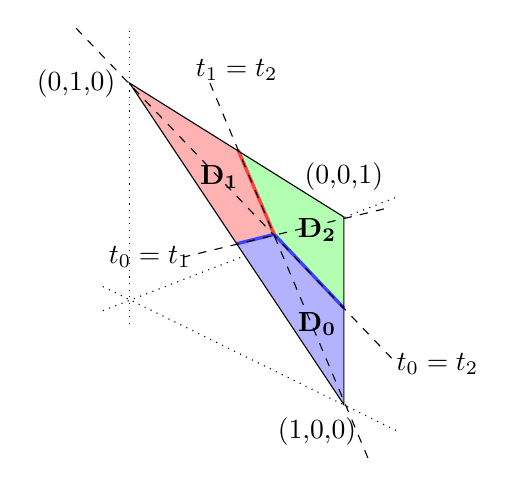
\begin{tikzpicture}[auto,scale = 1.7]
\draw[dotted] (0,0) -- (0,2.2);
\draw[dotted] (-0.2,0.1) -- (2,0.95);
\draw[dotted] (-0.2,0.28) -- (2,-0.8);
%\draw (-0.1,1.8) -- (0.1,1.8);
\node at (-0.4,1.8) {(0,1,0)};
%\draw (1.5,-0.65) -- (1.7,-0.55);
\node at (1.4,-0.80) {(1,0,0)};
%\draw (1.5,0.85) -- (1.7,0.75);
\node at (1.6,1.1) {(0,0,1)};
\node at (2.3,-0.3) {$t_0 = t_2$};
\node at (0.8,1.9) {$t_1=t_2$};
\node at (0.15,0.5) {$t_0=t_1$};
\draw[draw = gray!0,fill = red!30] (0,1.8) -- (0.8,0.59) -- (1.08,0.67) -- (0.81,1.3) -- cycle;
\draw[draw = gray!0,fill = blue!30] (1.6,-0.6) -- (1.6,0.12) -- (1.08,0.67) -- (0.8,0.6) -- cycle;
\draw[draw = gray!0,fill = green!30] (1.6,0.8) -- (1.6,0.12) -- (1.08,0.67) -- (0.81,1.3) -- cycle;
\draw[red!75, very thick] (0.81,1.3) -- (1.08,0.67);
\draw[blue!75, very thick] (1.6,0.12) -- (1.08,0.67);
\draw[blue!75,very thick] (1.08,0.67) -- (0.8,0.6);
\draw (0,1.8) -- (1.6,-0.6) -- (1.6,0.8) -- cycle;
\draw[dashed] (-0.4,2.21) -- (2,-0.3);
\draw[dashed] (1.78,-1) -- (0.6,1.8);
\draw[dashed] (1.9,0.86) -- (0.4,0.5);
\node at (1.4,0) {$\mathbf{D_0}$};
\node at (0.67,1.1) {$\mathbf{D_1}$};
\node at (1.4,0.7) {$\mathbf{D_2}$};
\end{tikzpicture}
\begin{tikzpicture}
\draw[white] (0,0) rectangle (0.5,1);
\end{tikzpicture}
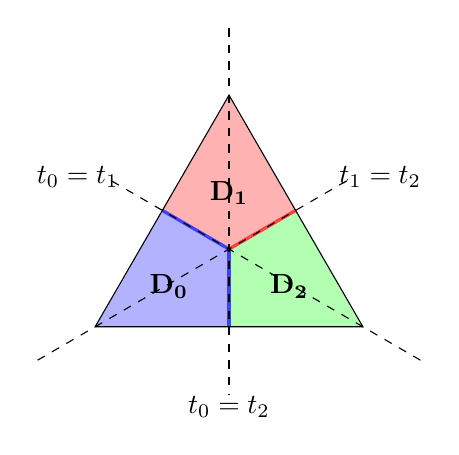
\begin{tikzpicture}[auto,scale = 1.7]
\node at (1,-0.6) {$t_0 = t_2$};
\node at (2.13,1.12) {$t_1=t_2$};
\node at (-0.13,1.12) {$t_0=t_1$};
\draw[white,fill = blue!30] (0,0) -- (0.5,0.87) -- (1,0.58) -- (1,0) -- cycle;
\draw[white,fill = red!30] (0.5,0.87) -- (1,1.73) -- (1.5,0.87) -- (1,0.58) -- cycle;
\draw[white,fill = green!30] (2,0) -- (1.5,0.87) -- (1,0.58) -- (1,0) -- cycle;
\draw[red!75,very thick] (1.5,0.87) -- (1,0.58);
\draw[blue!75,very thick] (0.5,0.87) -- (1,0.58);
\draw[blue!75,very thick] (1,0) -- (1,0.58);
\draw[dashed] (1,2.23) -- (1,-0.5);
\draw[dashed] (-0.43,-0.25) -- (1.93,1.12);
\draw[dashed] (2.43,-0.25) -- (0.07,1.12);
\draw (0,0) -- (1,1.73) -- (2,0) -- cycle;
\node at (0.55,0.3) {$\mathbf{D_0}$};
\node at (1.45,0.3) {$\mathbf{D_2}$};
\node at (1,1) {$\mathbf{D_1}$};
\end{tikzpicture}
\caption{2-dimensional structure $\vec\Delta_2$}
\end{center}
\end{figure}
We will say that a continuous map $\map{\gamma}{I}{\Delta_n}$ is a dipath of $\Delta_n$ if it is such that there exist $k \geq 1$, $0 \leq i_1 < \ldots < i_k \leq n$ integers and $0 < t_1 < \ldots < t_{k-1} < t_k = 1$ real numbers with :
\begin{itemize}
	\item $\forall t \in [0,t_1]$, $\gamma(t) \in D_{i_1}$ ;
	\item $\forall j \in \{2, \ldots, k\}$, $\forall t \in ]t_{j-1},t_j]$, $\gamma(t) \in D_{i_j}$.
\end{itemize}
Is it possible to prove that the induced geometric realization produces a d-space as wanted ?



\subsection*{Relation to persistency}


We have seen in Chapter 8 that even if intuitions from persistent homology seems similar to our computation of diagrams of homology, we cannot use directly techniques from persistency. Nevertheless, it would be interesting to look at what kind of informations persistency can give us on cubical complexes. For example, consider this cubical complex:
\begin{figure}[H]
\centering
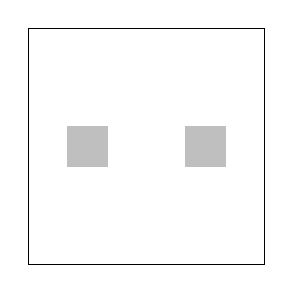
\begin{tikzpicture}[auto,scale = 1]
\draw (0,0) rectangle (3,3);
\draw [fill = gray!50,draw = gray!50] (0.5,1.25) rectangle (1,1.75);
\draw [fill = gray!50,draw = gray!50] (2,1.25) rectangle (2.5,1.75);
\end{tikzpicture}
\end{figure}
Persistency will be able to describe the evolution of the trace space between $0$ and $(t_1,t_2)$ by letting $t_1$ and $t_2$ evolve.
\begin{figure}[H]
		\centering
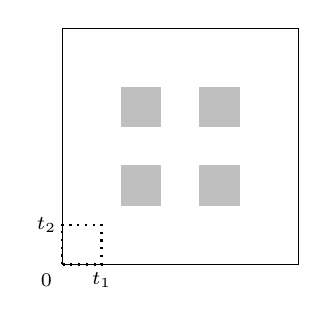
\begin{tikzpicture}[auto,scale = 1]
\draw (0,0) rectangle (3,3);
\draw [fill = gray!50,draw = gray!50] (0.75,0.75) rectangle (1.25,1.25);
\draw [fill = gray!50,draw = gray!50] (1.75,1.75) rectangle (2.25,2.25);
\draw [fill = gray!50,draw = gray!50] (0.75,1.75) rectangle (1.25,2.25);
\draw [fill = gray!50,draw = gray!50] (1.75,0.75) rectangle (2.25,1.25);
\draw [dotted, thick] (0,0) rectangle (0.5,0.5);
\node at (0.5,-0.2) {\scriptsize{$t_1$}};
\node at (-0.2,0.5) {\scriptsize{$t_2$}};
\node at (-0.2,-0.2) {\scriptsize{$0$}};
\end{tikzpicture}
\begin{tikzpicture}[auto,scale = 1]
\draw[draw = white] (0,0) rectangle (1.5,1.5);
\end{tikzpicture}
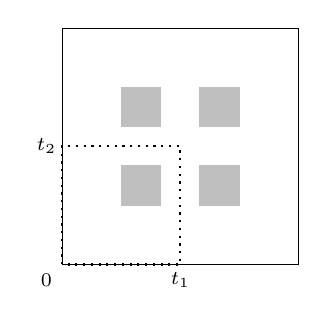
\begin{tikzpicture}[auto,scale = 1]
\draw (0,0) rectangle (3,3);
\draw [fill = gray!50,draw = gray!50] (0.75,0.75) rectangle (1.25,1.25);
\draw [fill = gray!50,draw = gray!50] (1.75,1.75) rectangle (2.25,2.25);
\draw [fill = gray!50,draw = gray!50] (0.75,1.75) rectangle (1.25,2.25);
\draw [fill = gray!50,draw = gray!50] (1.75,0.75) rectangle (2.25,1.25);
\draw [dotted, thick] (0,0) rectangle (1.5,1.5);
\node at (1.5,-0.2) {\scriptsize{$t_1$}};
\node at (-0.2,1.5) {\scriptsize{$t_2$}};
\node at (-0.2,-0.2) {\scriptsize{$0$}};
\end{tikzpicture}
\begin{tikzpicture}[auto,scale = 1]
\draw[draw = white] (0,0) rectangle (1.5,1.5);
\end{tikzpicture}
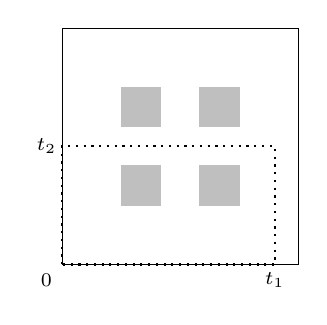
\begin{tikzpicture}[auto,scale = 1]
\draw (0,0) rectangle (3,3);
\draw [fill = gray!50,draw = gray!50] (0.75,0.75) rectangle (1.25,1.25);
\draw [fill = gray!50,draw = gray!50] (1.75,1.75) rectangle (2.25,2.25);
\draw [fill = gray!50,draw = gray!50] (0.75,1.75) rectangle (1.25,2.25);
\draw [fill = gray!50,draw = gray!50] (1.75,0.75) rectangle (2.25,1.25);
\draw [dotted, thick] (0,0) rectangle (2.7,1.5);
\node at (2.7,-0.2) {\scriptsize{$t_1$}};
\node at (-0.2,1.5) {\scriptsize{$t_2$}};
\node at (-0.2,-0.2) {\scriptsize{$0$}};
\end{tikzpicture}
\end{figure}
This uses $2$-dimensional persistency theory, but this essentially only look at how holes appear. We may be more interested by looking at trace spaces between $(t_1,t_2)$ and $(t_3,t_4)$ and see how it evolves when letting $t_1$, $t_2$, $t_3$ and $t_4$ evolve, using $4$-dimensional persistency.
\begin{figure}[H]
		\centering
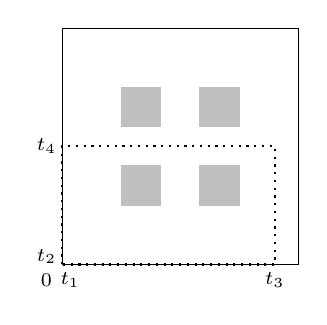
\begin{tikzpicture}[auto,scale = 1]
\draw (0,0) rectangle (3,3);
\draw [fill = gray!50,draw = gray!50] (0.75,0.75) rectangle (1.25,1.25);
\draw [fill = gray!50,draw = gray!50] (1.75,1.75) rectangle (2.25,2.25);
\draw [fill = gray!50,draw = gray!50] (0.75,1.75) rectangle (1.25,2.25);
\draw [fill = gray!50,draw = gray!50] (1.75,0.75) rectangle (2.25,1.25);
\draw [dotted, thick] (0,0) rectangle (2.7,1.5);
\node at (2.7,-0.2) {\scriptsize{$t_3$}};
\node at (-0.2,1.5) {\scriptsize{$t_4$}};
\node at (0.1,-0.2) {\scriptsize{$t_1$}};
\node at (-0.2,0.1) {\scriptsize{$t_2$}};
\node at (-0.2,-0.2) {\scriptsize{$0$}};
\end{tikzpicture}
\begin{tikzpicture}[auto,scale = 1]
\draw[draw = white] (0,0) rectangle (1.5,1.5);
\end{tikzpicture}
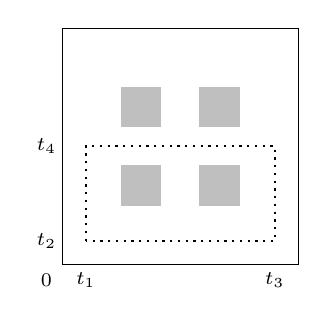
\begin{tikzpicture}[auto,scale = 1]
\draw (0,0) rectangle (3,3);
\draw [fill = gray!50,draw = gray!50] (0.75,0.75) rectangle (1.25,1.25);
\draw [fill = gray!50,draw = gray!50] (1.75,1.75) rectangle (2.25,2.25);
\draw [fill = gray!50,draw = gray!50] (0.75,1.75) rectangle (1.25,2.25);
\draw [fill = gray!50,draw = gray!50] (1.75,0.75) rectangle (2.25,1.25);
\draw [dotted, thick] (0.3,0.3) rectangle (2.7,1.5);
\node at (2.7,-0.2) {\scriptsize{$t_3$}};
\node at (-0.2,1.5) {\scriptsize{$t_4$}};
\node at (0.3,-0.2) {\scriptsize{$t_1$}};
\node at (-0.2,0.3) {\scriptsize{$t_2$}};
\node at (-0.2,-0.2) {\scriptsize{$0$}};
\end{tikzpicture}
\begin{tikzpicture}[auto,scale = 1]
\draw[draw = white] (0,0) rectangle (1.5,1.5);
\end{tikzpicture}
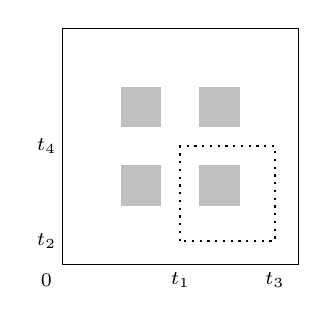
\begin{tikzpicture}[auto,scale = 1]
\draw (0,0) rectangle (3,3);
\draw [fill = gray!50,draw = gray!50] (0.75,0.75) rectangle (1.25,1.25);
\draw [fill = gray!50,draw = gray!50] (1.75,1.75) rectangle (2.25,2.25);
\draw [fill = gray!50,draw = gray!50] (0.75,1.75) rectangle (1.25,2.25);
\draw [fill = gray!50,draw = gray!50] (1.75,0.75) rectangle (2.25,1.25);
\draw [dotted, thick] (1.5,0.3) rectangle (2.7,1.5);
\node at (2.7,-0.2) {\scriptsize{$t_3$}};
\node at (-0.2,1.5) {\scriptsize{$t_4$}};
\node at (1.5,-0.2) {\scriptsize{$t_1$}};
\node at (-0.2,0.3) {\scriptsize{$t_2$}};
\node at (-0.2,-0.2) {\scriptsize{$0$}};
\end{tikzpicture}
\end{figure}





